% Encoding: ISO8859-1

% Based on thesisclass.cls of Timo Rohrberg, 2009
\documentclass{iti-seminar}

% Main document

% Packages
\usepackage[T1]{fontenc}
\usepackage[latin1]{inputenc} % Input in ISO 8859-1 (Latin1)

\usepackage{graphicx}
\usepackage{listings}
\usepackage{wrapfig}
\usepackage{subfigure}
\usepackage{url}

\usepackage{latexsym}
\usepackage{amstext}
\usepackage{amsfonts}
\usepackage{amssymb}
\usepackage{amsmath}

% Definitions
\newcites{Niklaus}{References} % Please set NAME to your name
\newcommand{\seminartitle}{Gems of Theoretical Computer Science}
\newcommand{\seminarsubject}{LOGSPACE, RandomWalks on Graphs and Universal Traversal Sequences}

% PDF file data
\hypersetup{
 pdftitle={\seminartitle}
}

% Start of main document
\begin{document}

\frontmatter
%% Encoding: ISO8859-1 %%

%% titlepage.tex

\def\usesf{}
\let\usesf\sffamily % uncomment this line for normal TeX font

\begin{titlepage}

\setlength{\unitlength}{1pt}
\begin{picture}(0,0)(160,770)
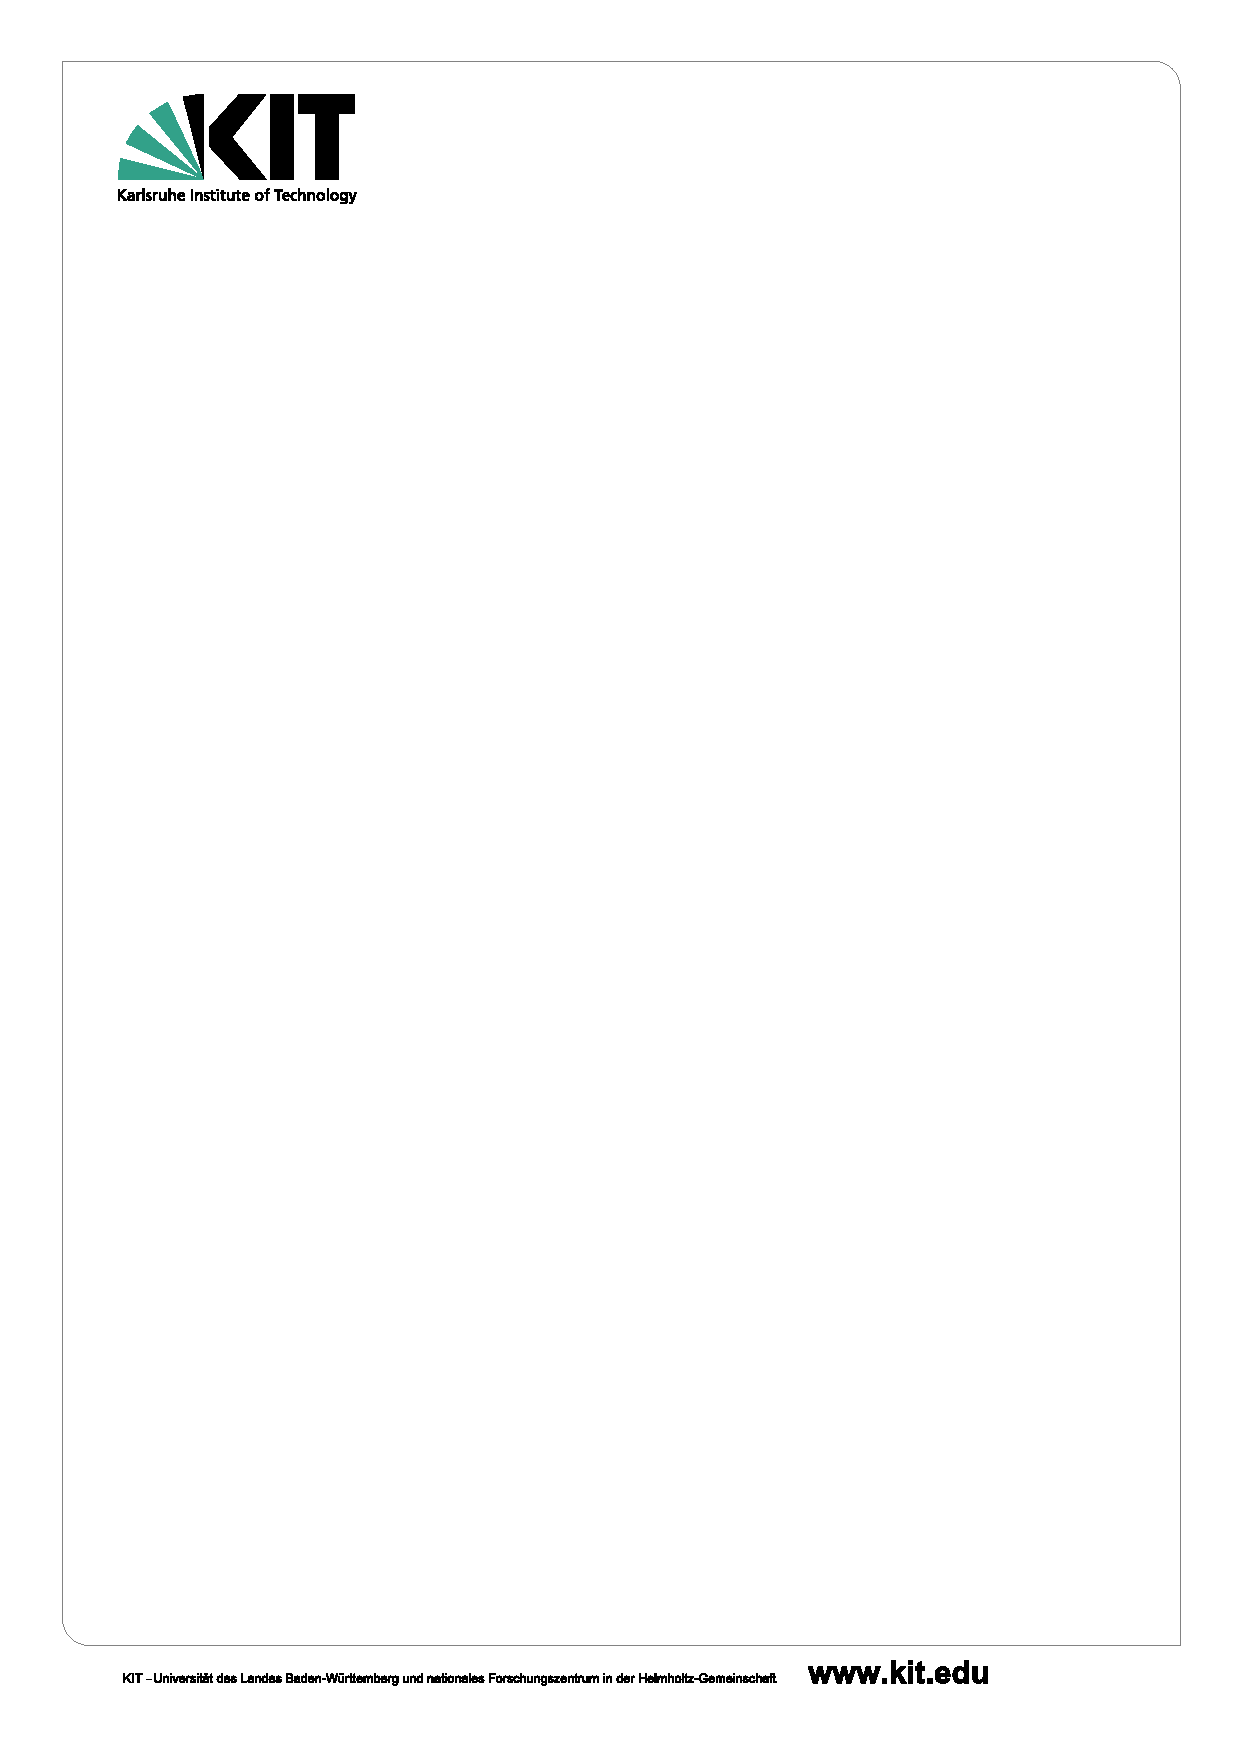
\includegraphics[width=\paperwidth]{logos/KIT_Deckblatt.pdf}
\end{picture}

\thispagestyle{empty}

\begin{center}
\hbox{}
\vfill
{\usesf
{\huge\bfseries Seminar\\
              \seminartitle \par }
{\large \seminarsubject \par}
\vskip 1.8cm
{\Large Summer term 2014\\}
\vskip 1cm

\vskip 1.2cm
Institute of Theoretical Informatics (ITI)\\
Department of Informatics\\
Karlsruhe Institute of Technology (KIT)\\
\vskip 3cm
\begin{tabular}{p{20mm}l}
Author: & {\usesf Patrick~Niklaus} \\
Betreuer: & {\usesf Jun.-Prof.\,Dr.~Henning~Meyerhenke} % Please specify advisers here
\end{tabular}
}
\end{center}
\vfill
\end{titlepage}

\thispagestyle{empty}
\ \vfill
\begin{flushleft}
  Copyright \(\copyright\) 2014 ITI and Patrick Niklaus\\ % Please set AUTHOR to your full name
  \ \\
  Institute of Theoretical Informatics (ITI)\\
  Department of Informatics\\
  Karlsruhe Institute of Technology\\
  Am Fasanengarten 5\\
  76128 Karlsruhe
\end{flushleft}
\newpage


\pagenumbering{roman}
\tableofcontents

% Main part
\mainmatter
{\includeTeX{Niklaus/RandomWalk}\relax} % please set NAME to your name and TITLE to the title of your work

\end{document}
